% ==============================================================================
% TCC - Nome do Aluno
% Capítulo 3 - Projeto Arquitetural e Implementação
% ==============================================================================
\chapter{Algoritmos Dinâmicos}
\label{sec-dinamicos}

\section{Grafos Dinâmicos}
\label{sec-dinamicos-grafos}
Os algoritmos apresentados até agora tratam apenas de grafos estáticos, ou seja, grafos em que o peso de suas arestas não mudam. Mas em situações reais podemos ter casos em que a modelagem feita por grafos requer que os pesos de suas arestas variem com o tempo. Para esses casos, temos grafos ditos \textbf{dinâmicos}. Exemplos de modelagem por grafos dinâmicos são o sistema de tempo real de trânsito em que os pesos das arestas correspondem ao tempo médio para percorrer um determinado trecho e esse tempo está diretamente ligado ao trânsito local em uma determinada hora; e o fluxo de em uma rede interna onde as arestas representam o caminho entre roteadores e os seus pesos correspondem ao uso desta linha, ou seja, o quão congestionada está.

Para calcularmos o menor caminho entre dois vértices em grafos dinâmicos, poderíamos utilizar os algoritmos de Dijsktra e A* (discutidos nos capítulos \ref{sec-dijkstra} e \ref{sec-aestrela})  para acharmos a rota, e quando houver uma detecção de mudança do peso de arestas, recalcularíamos novamente o trajeto reutilizando esses algoritmos. Em geral desejamos (ou necessitamos) que esse recálculo seja mais rápido. Para esse fim existem os algoritmos dinâmicos que calculam uma solução rápida porém não garantidamente ótima (elas são ditas sub-ótimas).

Exemplos de algoritmos são o D* \cite{stentz1994optimal}, D* Lite \cite{koenig2002d} e o AD* \cite{likhachev2008anytime}.

Será discutidos os algoritmos ARA* e AD* \cite{likhachev2008anytime}, que foram escolhidos para serem estudados por este trabalho.
\section{Algoritmo ARA*}
\label{sec-dinamicos-ara}

O algoritmo ARA* proposto em \citeonline{likhachev2008anytime}, está descrito nos algoritmos \ref{lst-dinamicos-ara-computepath}, \ref{lst-dinamicos-ara-key} e \ref{lst-dinamicos-ara-main}.

\begin{lstlisting}[mathescape, label=lst-dinamicos-ara-computepath, caption=Algoritmo ARA* - função de cálculo de caminho, float=htpb]
procedure ComputePath()
	while(key($s_{goal}$) > $min_{s \in OPEN(key(s))}$)
		remove s with smallest key(s) from OPEN;
		v(s) = g(s); CLOSED = CLOSED $\cup$ {s};
		for each successor s' of s
			if s' was never visited by ARA* before then
				v(s') = g(s') = $\infty$;
			if g(s') > g(s) + c(s, s')
				g(s') = g(s) + c(s, s');
				if s' $\notin$ CLOSED
					insert/update s' in OPEN with key(s');
				else
					insert s' into INCONS;
\end{lstlisting}

 
\begin{lstlisting}[mathescape, label=lst-dinamicos-ara-key, caption=Algoritmo ARA* - função da chave ordenadora da fila de prioridades, float=htpb]
procedure key(s)
	return g(s) + $\epsilon$ * h(s);
\end{lstlisting}

\begin{lstlisting}[mathescape, label=lst-dinamicos-ara-main, caption=Algoritmo ARA* - função principal, float=htpb]
procedure Main()
	g($s_{goal}$) = v($s_{goal}$) = $\infty$; v($s_{start}$) = $\infty$;
	g($s_{start}$) = 0; OPEN = CLOSED = INCONS = $\emptyset$;
	insert $s_{start}$ into OPEN with key($s_{start}$);
	ComputePath();
	publish current $\epsilon$-suboptimal solution;
	while $\epsilon > 1$
		decrease $\epsilon$;
		Move states from INCONS into OPEN
		Update the priorities for all s $\in$ OPEN according to key(s);
		CLOSED = $\emptyset$;
		ComputePath();
		publish current $\epsilon$-suboptimal solution;
\end{lstlisting}

A função principal é descrita no Algoritmo \ref{lst-dinamicos-ara-main}. Temos as variáveis g(s) e v(s) que correspondem ao valor da distância real calculada da origem $s_{start}$ até o vértice s (o valor de v(s), apesar de estar descrito no algoritmo conforme a literatura de origem, não é utilizado pelo algoritmo. Ela é utilizada, na verdade, no próximo algoritmo, AD*, que está descrito no mesmo artigo do ARA* e foi do critério de seus autores originais colocar essa variável em sua descrição. Portanto será ignorado na explicação que se segue). O valor de g($s_{goal}$) (distância real calculada da origem ao vértice destino) é atribuído como $\infty$ (infinito)\footnote{Vide nota de rodapé da seção \ref{sec-dijkstra-algoritmo}.}, enquanto que o valor de g($s_{start}$) é atribuído com o valor 0 (já que o valor da distancia real é calculada a partir da origem). Em seguida são criados os conjuntos ``OPEN'', ``CLOSED'' e ``INCONS'', correspondendo respectivamente ao conjunto dos ``ABERTOS'', ``FECHADOS'' e ``INCONSISTENTES''. O vértice $s_{start}$ é inserido na fila de prioridades do conjunto OPEN utilizando a função de chave ordenadora descrito no algoritmo \ref{lst-dinamicos-ara-key}. Essa função utiliza a estratégia da heurística inflada (descrito a seguir, na subseção \ref{sec-dinamicos-ad-consideracoes}).

A função de cálculo de caminho é então acionada pela função principal (algoritmo \ref{lst-dinamicos-ara-computepath}). Nesta função, o processo iterativo se faz enquanto o valor da chave de $s_{goal}$ for maior do que o valor da chave do termo mínimo da fila de prioridades. Enquanto isso for verdade, o vértice s, que corresponde ao valor do vértice com menor chave de OPEN, é removido deste e adicionado ao conjunto CLOSED. Para cada s' (que representa um vértice do conjunto de vértices adjacentes de s) é verificado se o mesmo já foi visitado pelo algoritmo e em caso negativo, o seu valor de g(s') é atribuído como $\infty$ (infinito). Em seguida, é verificado se a distância calculada até o momento para s', g(s'), é maior do que a soma de g(s) com o peso da aresta entre s e s'. Se caso positivo, g(s') é atualizado com esse novo valor. Em seguida é verificado se o vértice s' não pertence ao conjunto dos fechados e em caso positivo, ele é adicionado/atualizado no conjunto OPEN de acordo com a função de chave ordenadora. Caso contrário, ele é adicionado ao conjunto dos INCONS.

Após o cálculo do caminho e de acordo com função principal (algoritmo \ref{lst-dinamicos-ara-main}), a solução $\epsilon$ sub-ótima (a explicação do motivo de a solução ser sub-ótima será dada na subseção \ref{sec-dinamicos-ara-consideracoes}) é apresentada pelo algoritmo. A partir daí começa o processo iterativo em que se verifica se o valor de $\epsilon$ é maior que 1. Em caso positivo, o valor de $\epsilon$ é decrescido por um fator de corte estipulado como parâmetro de entrada. Os vértices pertencentes a INCONS são movidos para OPEN e todas as chaves da fila de prioridades são atualizadas considerando o novo valor de $\epsilon$. O conjunto CLOSED é esvaziado e a função de cálculo de caminho é acionada novamente e seu respectivo resultado é apresentado.

\subsection{Heurística inflada e considerações sobre o algoritmo}
\label{sec-dinamicos-ara-consideracoes}

A principal diferença entre o algoritmo ARA* e o A* está na utilização da estratégia da heurística inflada. Ela consiste em utilizar a mesma função de ordenação de chaves da fila de prioridades do algoritmo A*, com a exceção de que o valor heurístico é multiplicado por um fator $\epsilon$. Isso faz com que menos vértices sejam visitados, já que os menos ``promissores'' serão posicionados mais para o final da fila de prioridades enquanto que os mais ``promissores'' serão posicionados mais para frente, e com isso é mais provável que um caminho até o vértice destino, $s_{goal}$, seja encontrado mais rápido do que pelo algoritmo A* (já que menos vértices deverão ser visitados). Entretanto, ao se utilizar esta técnica perdemos a garantia do resultado ótimo do algoritmo (algo semelhante ao que ocorre quando não utilizamos heurísticas não-admissíveis. Vide subseção \ref{sec-aestrela-algoritmo-heuristica}).

Porém, uma grande vantagem de se utilizar essa estratégia é que teremos um limite superior para a solução encontrada. Considere que o custo ótimo de um determinado caminho seja C*. Se o utilizarmos a função g( s ) + $\epsilon$ * h( s ), com o valor de $\epsilon > 1$, então há a garantia de que a nova solução C, C* $\leq$ C $\leq \epsilon$ x C*. Com isso, se $\epsilon$ = 1, a solução encontrada será garantidamente ótima \cite{moura2010estudo}.

Portanto a ideia principal é achar uma solução rápida, porém não-garantidamente ótima, atribuindo um valor $\epsilon$ maior do que 1, e caso a aplicação permita o uso de um tempo maior para aprimorarmos o resultado\footnote{Por exemplo, uma determinada aplicação necessita que se ache um caminho em no máximo 2 segundos. Se o algoritmo achar uma solução sub-ótima em 3 ms, dispomos de mais 1997 ms para podermos aprimorar ela.}, diminuímos o valor de $\epsilon$. E se o tempo ainda permitir, diminuímos até termos $\epsilon$ = 1, em que a solução será garantidamente ótima. 
\newpage
Outra estratégia utilizada para ganhar tempo, a cada novo valor de $\epsilon$ em que a função para cálculo de caminho é acionada (algoritmo \ref{lst-dinamicos-ara-computepath}), não é necessário recalcular todos os vértices visitados anteriormente, já que os mesmos permanecem na lista de abertos (tendo apenas suas chaves atualizadas com o novo valor de $\epsilon$ e consequentemente a ordem dos vértices também é reconfigurada de acordo com esses novos valores). Além disso, caso haja um melhor caminho encontrado para um vértice que pertence aos fechados, este são colocados em INCONS dos quais serão enviados para OPEN para serem recalculados na próxima busca (a busca se refere ao número da iteração da invocação da função de cálculo de caminho, contido no algoritmo \ref{lst-dinamicos-ara-computepath}, e consequentemente ao valor de $\epsilon$ a ele atribuído).

A figura \ref{fig-ara-exemplo}, contida em \citeonline{likhachev2008anytime}, mostra a aplicação da estratégia da heurística inflada com seus respectivos resultados encontrados pelo algoritmo.

\begin{figure}[H]
\centering
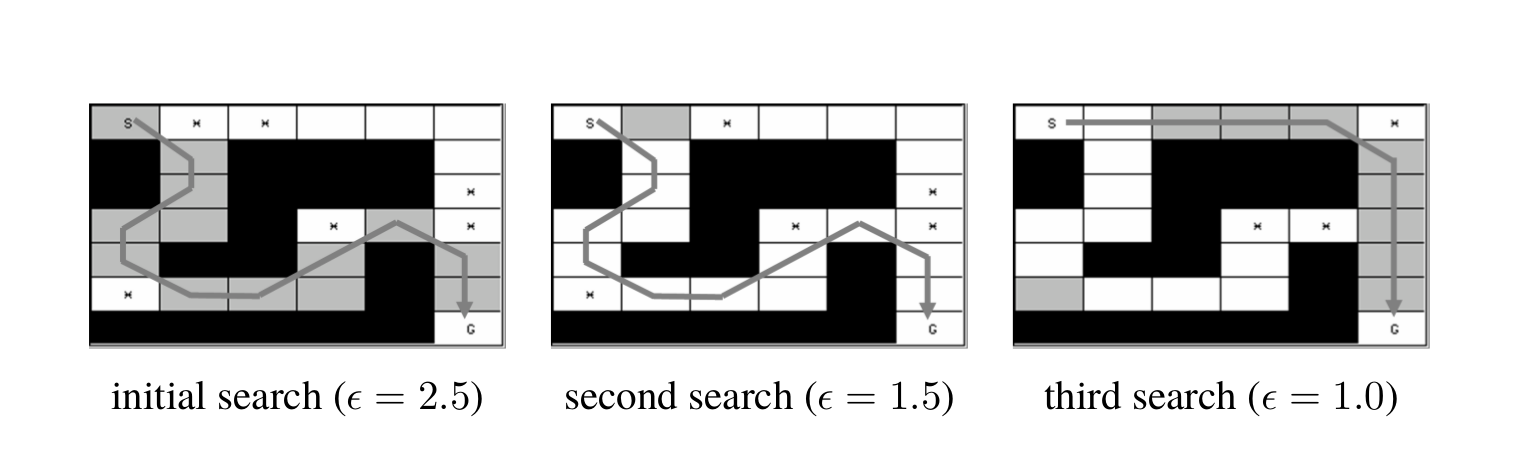
\includegraphics[width=.80\textwidth]{figuras/ara-3} 
\caption{Exemplo de aplicação da estratégia de diminuição do valor de $\epsilon$.}
\label{fig-ara-exemplo}
\end{figure}
\section{Algoritmo AD*}
\label{sec-dinamicos-ad}

O algoritmo AD* também proposto em \citeonline{likhachev2008anytime}, está descrito nos algoritmos \ref{lst-dinamicos-ad-set}, \ref{lst-dinamicos-ad-computepath}, \ref{lst-dinamicos-ad-key} e \ref{lst-dinamicos-ad-main}.

\begin{lstlisting}[mathescape, label=lst-dinamicos-ad-set, caption=Algoritmo AD* - função para determinar o conjunto ao qual vértice pertencerá, float=htpb]
procedure UpdateSetMembership(s)
	if ($v(s) \neq g(s)$)
		if (s $\notin$ CLOSED) insert/update s in OPEN with key(s);
		else if (s $\notin$ INCONS) insert s in INCONS;
	else
		if (s $\in$ OPEN) remove s from OPEN;
		else if (s $\in$ INCONS) remove s from INCONS;
\end{lstlisting}

\begin{lstlisting}[mathescape, label=lst-dinamicos-ad-computepath, caption=Algoritmo AD* - função de cálculo de caminho, float=htpb]
procedure ComputePath()
	while(key($s_{goal}$) > $min_{s \in OPEN(key(s))}$ OR v($s_{goal}$) < g($s_{goal}$)) 
		remove s with smallest key(s) from OPEN;
		if v(s) > g(s)
			v(s) = g(s); CLOSED = CLOSED $\cup$ {s};
			for each successor s' of s
				if s' was never visited by AD* before then
					v(s') = g(s') = $\infty$;bp(s') = null;
				if g(s') > g(s) + c(s, s')
					g(s') = g(s) + c(s, s');
					bp(s') = s;
					g(s') = g(bp(s')) + c(bp(s'),s'); UpdateSetMembership(s');
		else
			v(s) = $\infty$; UpdateSetMembership(s);
			for each successor s' of s
			if s' was never visited by AD* before then
				v(s') = g(s') = $\infty$;bp(s') = null;
			if bp(s') = s
				bp(s') = $argmin_{s'' \in pred(s')}$ v(s'') + c(s'',s');
				g(s') = v(bp(s')) + c(bp(s'),s'); UpdateSetMembership(s');
\end{lstlisting}

\begin{lstlisting}[mathescape, label=lst-dinamicos-ad-key, caption=Algoritmo AD* - função da chave ordenadora da fila de prioridades, float=htpb]
procedure key(s)
	if (v(s) $\geq$ g(s))
		return [g(s) + $\epsilon$ * h(s); g(s)];
	else
		return [v(s) + h(s); v(s)];
\end{lstlisting}

\begin{lstlisting}[mathescape, label=lst-dinamicos-ad-main, caption=Algoritmo AD* - função principal, float=htpb]
procedure Main()
	g($s_{goal}$) = v($s_{goal}$) = $\infty$; v($s_{start}$) = $\infty$;bp($s_{goal}$) = bp($s_{start}$) = null;
	g($s_{start}$) = 0; OPEN = CLOSED = INCONS = $\emptyset$; $\epsilon = \epsilon_{0}$;
	insert $s_{start}$ into OPEN with key($s_{start}$);
	forever
		ComputePath();
		publish current $\epsilon$-suboptimal solution;
		if $\epsilon = 1$
			wait changes in edge costs;
		for all directed edges (u,v) with changed edge costs
			update the edge cost c(u,v);
			if ( $v \neq s_{start}$ AND v was visited by AD* before)
				bp(v) = $argmin_{s'' \in pred(v)}$ v(s'') + c(s'',v);
				g(v) = v(bp(v)) + c(bp(v),v); UpdateSetMembership(v);
		if significant edge cost changes were observed
			increase $\epsilon$ or re-plan from scratch (i.e., re-excute Main function);
		else if $\epsilon > 1$
			decrease $\epsilon$;
		Move states from INCONS into OPEN
		Update the priorities for all s $\in$ OPEN according to key(s);
		CLOSED = $\emptyset$;
\end{lstlisting}

O algoritmo é muito semelhante em sua execução ao ARA*, já que o AD* é uma adaptação do mesmo \cite{moura2010estudo}. A função principal (algoritmo \ref{lst-dinamicos-ad-main}) começa iniciando os valores de g($s_{goal}$), v($s_{goal}$) e v($s_{start}$) como $\infty$, bp($s_{start}$) como ponteiro nulo e g($s_{start}$) como 0. Em seguida o vértice $s_{start}$ é inserido na fila de prioridades de acordo com  a função de chave ordenadora descrita no algoritmo \ref{lst-dinamicos-ad-key}. Disso, é acionado a função de cálculo de caminho (algoritmo \ref{lst-dinamicos-ad-computepath}).

Essa função trabalha da seguinte forma: inicialmente se verifica se o valor da chave de $s_{goal}$ é maior do que a menor chave da fila de prioridades (condição semelhante ao do algoritmo ARA*, vide algoritmo \ref{lst-dinamicos-ara-computepath}) ou se o valor de v($s_{goal}$) é menor do que o valor de g( $s_{goal}$ ). Caso seja verdade, o processo iterativo é iniciado. O vértice s, que corresponde ao vértice com menor chave na fila de prioridades é removido do conjunto OPEN, e é verificado se o valor de v(s) é maior do que o g(s), ou seja, se o valor da distância calculada da busca anterior é maior do que o valor da busca atual (esse é o caso padrão do algoritmo). Sendo verdade, o algoritmo segue a mesma forma de execução do ARA*, conforme descrito na seção \ref{sec-dinamicos-ara}. A diferença de tratamento ocorre quando a condição inicial não ocorre, e neste caso, o valor de v( s ) é atualizado como $\infty$, e para cada vértice s' adjacente de s é verificado se este já havia sido visitado pelo algoritmo. Caso contrário, os valores de v( s' ), g( s' ) são iniciados como $\infty$ e bp( s') é iniciado como ponteiro nulo. Em seguida, é verificado se bp( s' ) é igual ao vértice s. Em caso positivo, o bp( s' ) é atualizado com o vértice predecessor de s', s'', cujo valor da função v(s'') + c( s'', s') é a menor dentre todos os vértices predecessores de s'. Feito isso, o valor de g( s' ) é atualizado com esse novo valor. Finalmente a função de determinação para qual conjunto pertencerá s' é chamada (função ``UpdateSetMembership'').

A função de determinação ao qual conjunto pertencerá funciona de uma maneira muito simples. Caso os valores de v( s ) e g( s ) sejam diferentes, a função tem comportamento similar ao processo de atribuição de conjunto do ARA* (vide algoritmo \ref{lst-dinamicos-ara-computepath}). A diferença ocorre quando esses valores são iguais (ou seja, não houve mudança de valores entre a busca atual e a anterior). O vértice é removido de OPEN caso pertença a ele ou removido de INCONS caso pertença a este. Isso feito para que este vértice não precise ser explorado nesta busca ou na próxima (caso esteja em INCOS).

Voltando ao método principal (algoritmo \ref{lst-dinamicos-ad-main}), a função segue o mesmo padrão da ARA*. A única exceção se dá quando mudanças no grafo são detectadas (mudança dos pesos das arestas). Neste caso, para cada aresta (u,v) mudada, é atribuído ao valor bp( v ), o vértice s'', predecessor de v, cuja função v( s'' ) + c( s'', v) seja mínima. Consequentemente, o valor de g( v ) é atualizado conforme esse valor e a função de atribuição de conjunto é acionada. 